\subsubsection{Perinatal Deaths vs Mothers' Age}
Perinatal deaths can also happen because of mothers' health factors such as age. To identify how age is contributing to perinatal death we have generated \textbf{Figure \ref{fig:peri_mother}} to try to understand the trend of the data. We can see that perinatal death is significantly high among mothers who are aged below 20. The second biggest group, in this case, is mothers who are aged 40 and over. The group that has consistently low perinatal death is mothers who are aged between 30-34.
\begin{figure}
  \centering
  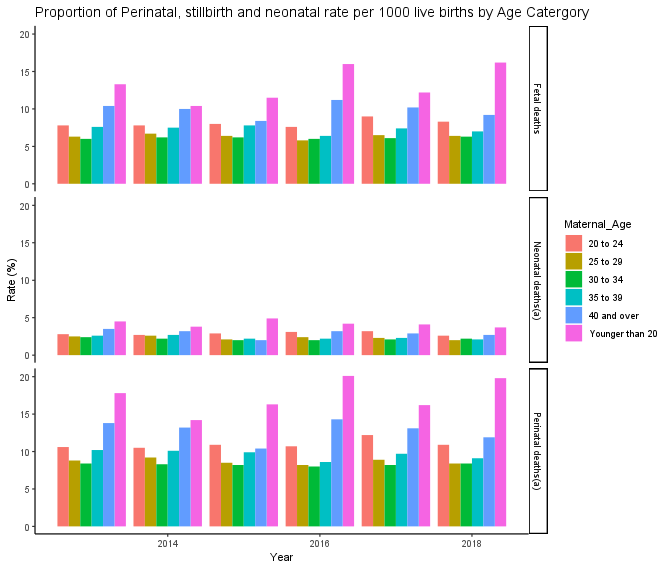
\includegraphics[width=.75\textwidth]{subsections/perinatal_deaths/by_mother_age_baby_death.png}
  \caption{Perinatal death vs Maternal age}
  \label{fig:peri_mother}
\end{figure}